\documentclass{article}

\usepackage[left=0.7in,
            right=0.7in,
            top=0.5in,
            bottom=0.7in]{geometry}
\usepackage{graphicx}
\usepackage{amsmath}
\usepackage{caption}

\begin{document}

\section{Course content}
\begin{itemize}
    \item supervised, unpservised, reinforcement learning. classification vs clustering, Example of supervised learning and others
    \item data space with examples, example of datasets, labels, data vs task vs loss, example of common losses
    \item test set vs validation set, model complexity, params vs hyperparams, overfitting, underfitting, example of overfitting, example of underfitting, causality vs correlation, example of causality, example of correlation, vbias/variance tradeoff and regularizations (lp norms, lasso ridge net)
    \item ripasso probabilita, probabilita condizionata, probabilita a posteriori, probabilita a priori, joint distribution, bayes th, i.i.d
    \item gradient descent (weights and learning rate)
    \item unsupervised learnign (manifold, desnity estimation, clustering, dimensionality reduction, flat clustering (partition and density based), fuzzy clustering, hierichical clustering)
\end{itemize}

\section{What is Machine Learning}
Artificial Intelligence is the overall umbrella term for the field of developing intelligent computer systems. Machine learning is a subfield of AI that focuses on developing algorithms that can learn from data.\\
In traditional computer science, algorithms are designed to follow a set of rules or logical steps to perform a specific task.
In contrast, machine learning algorithms are designed to optimize their performance based on a given objective or metric by adjusting their parameters.
Therefore, machine learning focuses more on optimization, while traditional computer science focuses more on logical problem solving and efficient algorithm design.\\
\noindent Machine learning is growing rapidly due to several factors:
\begin{itemize}
    \item Increasing availability of data: With the proliferation of digital devices and the internet, vast amounts of data are being generated every day. This data provides an opportunity for machine learning algorithms to learn from it and improve their performance.
    \item Advancements in computing power: Machine learning algorithms require a lot of computational resources, and recent advances in computing power have made it possible to train larger and more complex models than ever before.
    \item Improved algorithms and techniques: Machine learning research has made significant progress in developing new algorithms and techniques that are more accurate, efficient, and scalable than earlier methods.
    \item Business opportunities: Machine learning has the potential to unlock new business opportunities and create efficiencies in existing industries. Companies are increasingly adopting machine learning to automate tasks, optimize processes, and make better decisions.
    \item Availability of open-source tools and frameworks: The availability of open-source machine learning tools and frameworks such as TensorFlow, PyTorch, and scikit-learn has made it easier for developers to experiment with machine learning and build custom models.
    \item Interdisciplinary collaborations: Machine learning is a highly interdisciplinary field that draws on expertise from computer science, mathematics, statistics, and other domains. Collaboration between experts from different fields is driving innovation and expanding the boundaries of what's possible with machine learning.
\end{itemize}
These factors, among others, are contributing to the rapid growth of machine learning and its increasing adoption in various industries and domains.

\noindent Here are some applications of machine learning:
\begin{itemize}
    \item \textbf{Chemistry}: Machine learning is used to predict the properties of molecules, design new drugs, and improve the efficiency of chemical processes. It is also used in materials science to predict the behavior of materials and design new materials with specific properties.
    
    \item \textbf{Medicine}: Machine learning is used for medical diagnosis, personalized treatment plans, drug discovery, and clinical decision making. It is also used in healthcare management to optimize resource allocation and reduce costs.

    \item \textbf{Mathematics}: Machine learning is used to solve complex mathematical problems, such as optimization and numerical analysis. It is also used in data analysis and pattern recognition in various branches of mathematics, such as algebra, topology, and geometry.
    
    \item \textbf{Self-driving cars}: Machine learning algorithms are used to process sensor data and make decisions in real-time for autonomous vehicles. This includes object detection, tracking, and recognition, as well as route planning and decision making based on environmental conditions.
    
    \item \textbf{AlphaGo (DeepMind)}: Machine learning was used to develop the AlphaGo program, which became the first computer program to defeat a human world champion at the board game Go. This was a significant achievement in the field of artificial intelligence and demonstrated the potential of machine learning in complex decision making.
    
    \item \textbf{Image processing and computer vision}: Machine learning algorithms are used to detect and recognize objects and patterns in images and videos. This includes face recognition, object detection, and image segmentation. Machine learning is also used in 3D computer vision, such as reconstructing 3D models from multiple 2D images.
    
    \item \textbf{Natural language processing (NLP)}: Machine learning is used to analyze and generate human language. This includes tasks such as language translation, sentiment analysis, and speech recognition. NLP is used in various applications, such as virtual assistants, chatbots, and language learning tools.
    
    \item \textbf{Fraud detection}: Machine learning algorithms are used to detect and prevent fraudulent activities in various domains, such as finance, e-commerce, and insurance. This includes identifying patterns of fraudulent behavior and predicting the likelihood of fraudulent activities.
    
    \item \textbf{Recommendation systems}: Machine learning is used to build recommendation systems that suggest products, services, or content to users based on their preferences and behavior. This includes collaborative filtering, content-based filtering, and hybrid approaches.
    
    \item \textbf{Predictive maintenance}: Machine learning is used to predict equipment failure and maintenance needs in various industries, such as manufacturing, transportation, and energy. This includes analyzing sensor data and other parameters to predict when maintenance is needed to prevent equipment failure and reduce downtime.
    
    \item \textbf{AlphaFold}: Machine learning was used to develop the AlphaFold program, a computer program to predict the 3D structure of a protein from its amino acid sequence.
    \begin{figure}[!h]
        \centering
        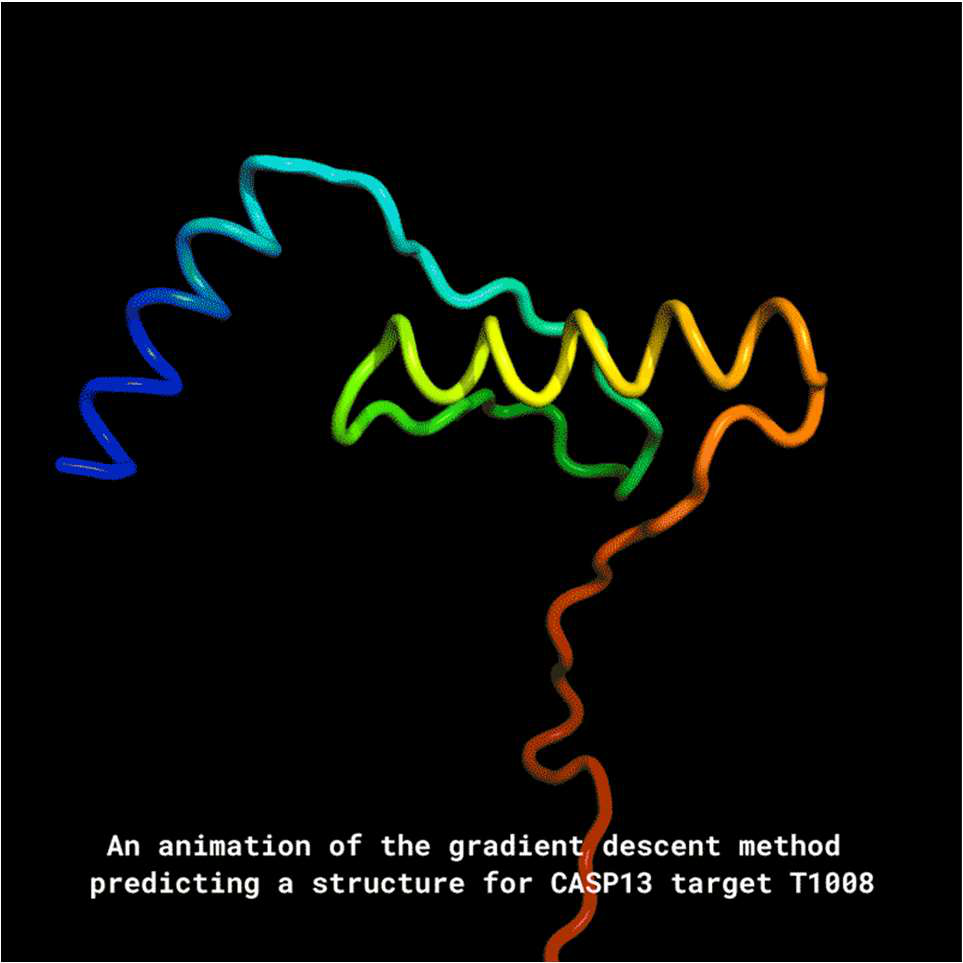
\includegraphics[width=4.5cm]{./images/p30_img183.png}
        \caption{AlphaFold}
    \end{figure}
\end{itemize}

\section{Machine Learning types}
\textbf{Supervised Learning:}
Supervised learning is a type of machine learning where the algorithm is trained on labeled data, where the correct output is provided for each input. The goal is to learn a function that maps inputs to outputs by finding patterns in the data. The algorithm can then use this function to make predictions on new, unseen data. Examples of supervised learning problems include:

\begin{itemize}
\item Classification: In classification, the goal is to predict a categorical variable based on a set of input features. For example, predicting whether an email is spam or not based on its content.
\item Regression: In regression, the goal is to predict a continuous variable based on a set of input features. For example, predicting the price of a house based on its size, location, and other features.
\end{itemize}
\textbf{Unsupervised Learning:}
Unsupervised learning is a type of machine learning where the algorithm is trained on unlabeled data, where the correct output is not provided. The goal is to find patterns or structure in the data without any prior knowledge of what the output should be. Examples of unsupervised learning problems include:

\begin{itemize}
\item Clustering: In clustering, the goal is to group similar data points together based on their features. For example, clustering customers based on their purchasing behavior to identify different market segments.
\item Dimensionality Reduction: In dimensionality reduction, the goal is to reduce the number of input features while preserving as much information as possible. For example, reducing the number of features in an image to make it easier to process.
\end{itemize}
\textbf{Reinforcement Learning:}
Reinforcement learning is a type of machine learning where the algorithm learns by interacting with an environment and receiving feedback in the form of rewards or penalties. The goal is to learn a policy that maximizes the cumulative reward over time. Examples of reinforcement learning problems include:

\begin{itemize}
\item Game Playing: In game playing, the goal is to learn a strategy that maximizes the chances of winning a game. For example, learning to play chess or Go.
\item Robotics: In robotics, the goal is to learn a policy that allows a robot to perform tasks in a dynamic environment. For example, learning to navigate a maze or pick up objects.
\end{itemize}
Overall, supervised, unsupervised, and reinforcement learning are three major categories of machine learning algorithms, each with their own characteristics and applications.\\
\textbf{Classification versus Clustering:}
\begin{itemize}
\item Classification: Classification is a type of supervised learning problem where the goal is to predict a categorical variable based on a set of input features. Examples include predicting whether an email is spam or not, or whether a patient has a particular disease based on their symptoms.
\item Clustering: Clustering is a type of unsupervised learning problem where the goal is to group similar data points together based on their features, without any prior knowledge of what the groups should be. Examples include clustering customers based on their purchasing behavior, or clustering genes based on their expression levels.
\end{itemize}
\begin{figure}[!ht]
    \centering
    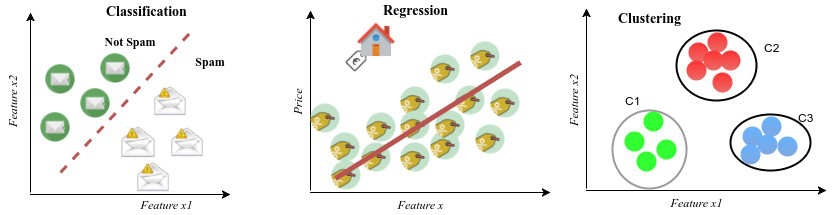
\includegraphics[width=\textwidth]{./images/p50_img275.png}
    \caption{Example of classification, regression, clustering}
\end{figure}
Classification and clustering are used for discrete data, where the input features are categorical or discrete values.\\
\section {Basic definitions}
The term \textbf{data space} refers to the set of all possible inputs that the model can receive.\\
On the other hand, the \textbf{label space} refers to the set of all possible outputs that the model can produce.\\\\
To give a concrete example, consider the CIFAR-10 dataset, which consists of 60,000 32x32 color images in 10 classes, with 6,000 images per class.
In this dataset, the data space would be the set of all possible 32x32 color images, while the label space would be the set of 10 possible classes: airplane, automobile, bird, cat, deer, dog, frog, horse, ship, and truck.
A machine learning model trained on this dataset would take an input image from the data space and produce an output label from the label space.\\\\
\begin{figure}[!ht]
    \centering
    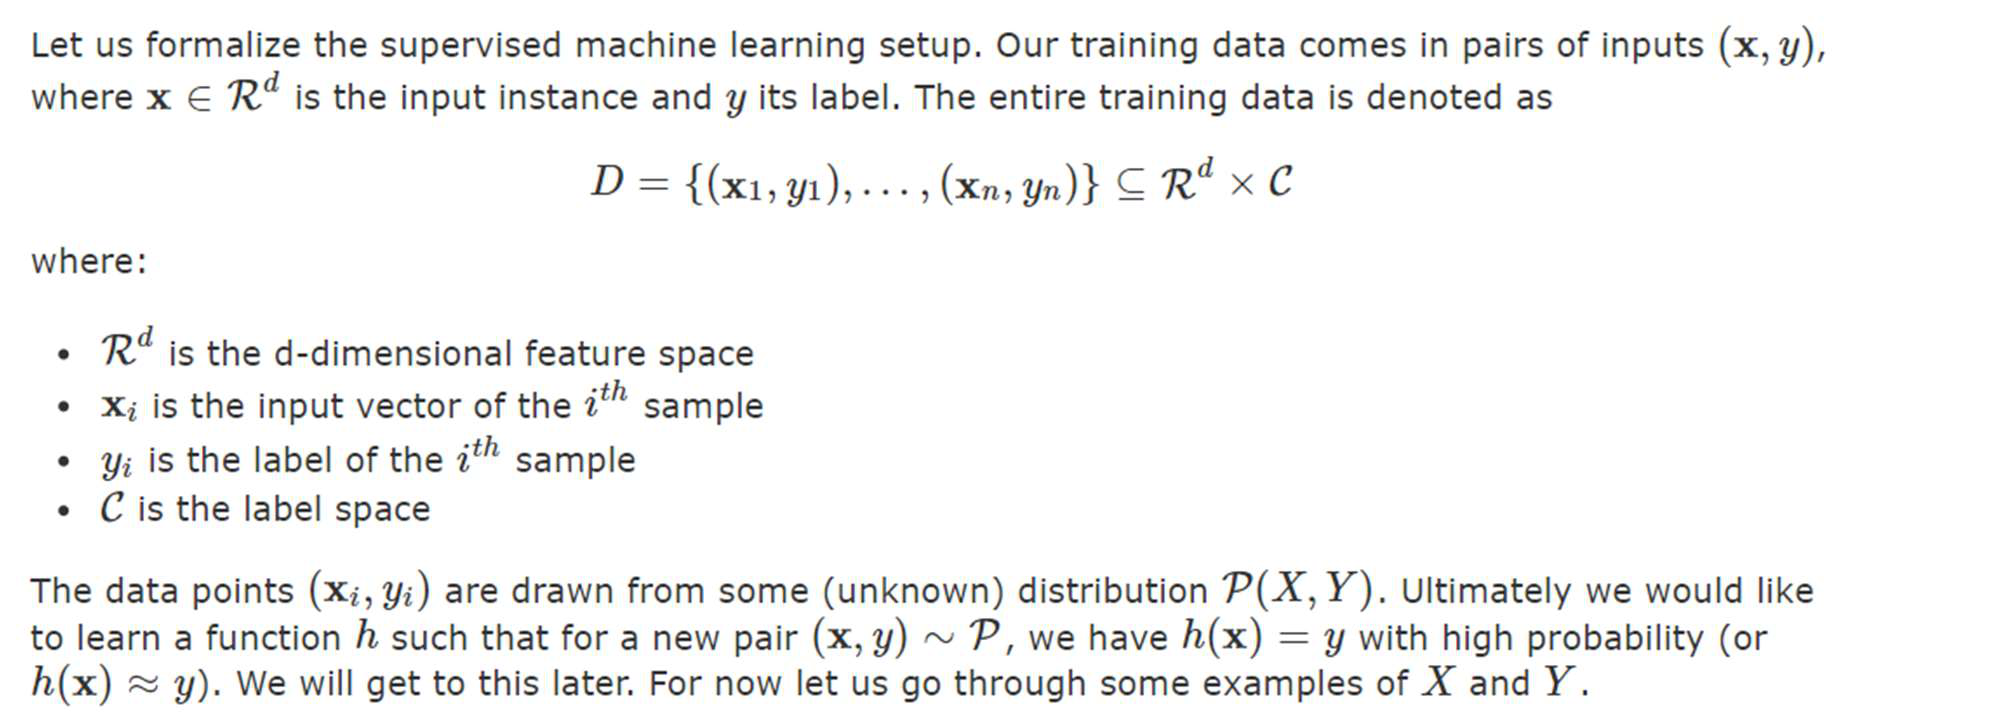
\includegraphics[width=\textwidth]{./images/p63_img322.png}
\end{figure}

\noindent The task refers to the goal of the machine learning model. For example, in an image classification problem, the task might be to correctly predict the label of an image given its input.\\
The model is a mathematical function that maps the input data to the output label.\\
The loss is a mathematical function that measures the difference between the predicted output of the model and the true output. The goal of training the model is to minimize this loss function.\\
Commonly used loss functions in machine learning include:
\begin{itemize}
    \item Mean squared error (MSE): Used for regression problems, the MSE measures the average squared difference between the predicted and true values.
    \[\text{MSE}=\frac{1}{N} \sum_{i=1}^N (y_i-\hat{y}_i)^2\]
    RMSE is the square root of MSE, which makes it easier to interpret because it is in the same units as the target variable but it is more sensitive to outliers than MSE. 
    \item Cross-entropy: Used for classification problems, cross-entropy measures the difference between the predicted and true probability distributions over the classes.
    \[\text{FORMULA}\]
    \item Binary cross-entropy: A variant of cross-entropy used for binary classification problems where there are only two possible classes.
    \[\text{FORMULA}\]
    \item Hinge loss: Used for classification problems in which the model is expected to produce a binary output, the hinge loss measures the difference between the predicted output and the true output.
    \[\text{FORMULA}\]
    \item KL divergence: Measures the difference between the predicted and true probability distributions over the classes or categories.
    \[\text{FORMULA}\]
\end{itemize}
\section{Dataset processing}
Splitting a dataset is a common practice in machine learning to evaluate the performance of a model and prevent overfitting. Typically, a dataset is split into two or three subsets: a training set, a validation set (sometimes), and a test set.\\
\begin{itemize}
    \item Training set: This subset of data is used to train the machine learning model. The model learns from the patterns in the training data and adjusts its parameters to minimize the loss function. This is the largest subset of data, typically around 70-80% of the total data, and should be representative of the underlying distribution of the data.
    \item Validation set: This subset of data is sometimes used to tune the hyperparameters of the model. Hyperparameters are settings of the model that are not learned from the data, such as the learning rate or the number of layers in a neural network. The validation set is not used for training, but instead provides a way to evaluate different choices of hyperparameters and select the best ones.
    \item Test set: This subset of data is used to evaluate the performance of the final model after it has been trained and tuned. The test set should be representative of the real-world data that the model will encounter in practice, and should not be used for training or tuning the model.
\end{itemize}
The goal is to ensure that the model is robust and generalizes well to new data.\\
\section{Model complexity and overfitting}
Model complexity refers to how flexible or expressive a machine learning model is in terms of its ability to capture patterns in the data. A simple model has a low level of complexity and may be easy to interpret, but may not capture all of the important patterns in the data.\\
A complex model, on the other hand, has a high level of complexity and may capture more of the patterns in the data, but may be harder to interpret and more prone to overfitting.\\\\
Overfitting occurs when a model is too complex and learns the noise or random variations in the training data, instead of the underlying patterns. This leads to poor generalization performance, where the model performs well on the training data but poorly on new, unseen data. An example of overfitting is a decision tree that has many levels and splits, which captures all the noise in the training data and does not generalize well to new data.\\\\
Underfitting occurs when a model is too simple and cannot capture the underlying patterns in the data, leading to poor performance on both the training and test sets. An example of underfitting is a linear regression model that tries to fit a non-linear relationship between the input and output variables, and does not capture the true pattern in the data.
\begin{figure}[!ht]
    \centering
    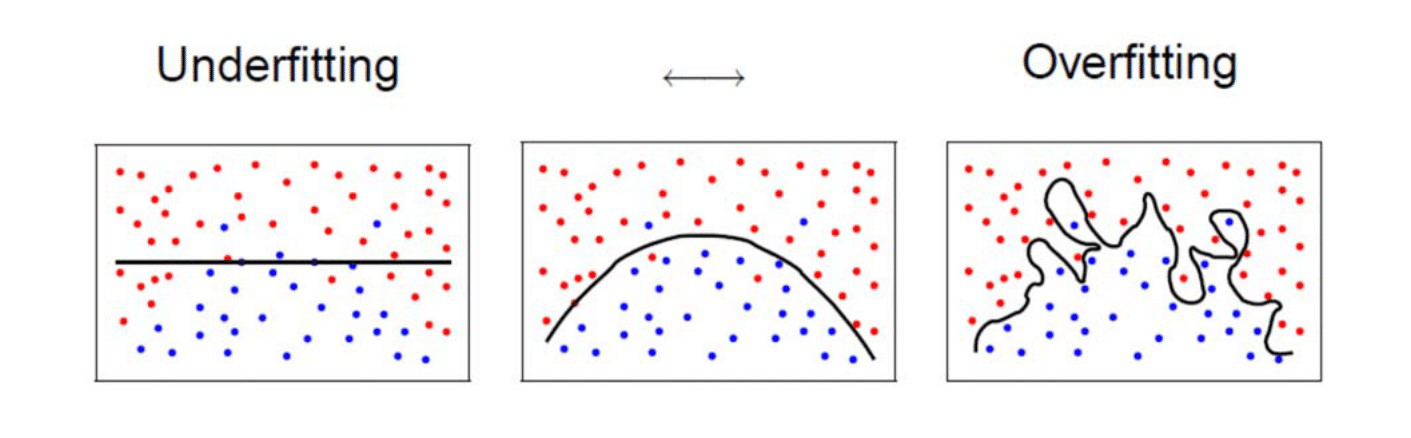
\includegraphics[width=\textwidth]{./images/p93_img447.png}
    \caption{Example of overfitting and underfitting}
\end{figure}

\[\text{TODO INSERT EXAMPLE OF LIN. REGRESS. TO A CURVE}\]
\newpage
\section{Bias-variance tradeoff}
The bias-variance tradeoff is the balance between the complexity of the model and its ability to generalize well to new data.\\
\begin{figure}[!ht]
    \centering
    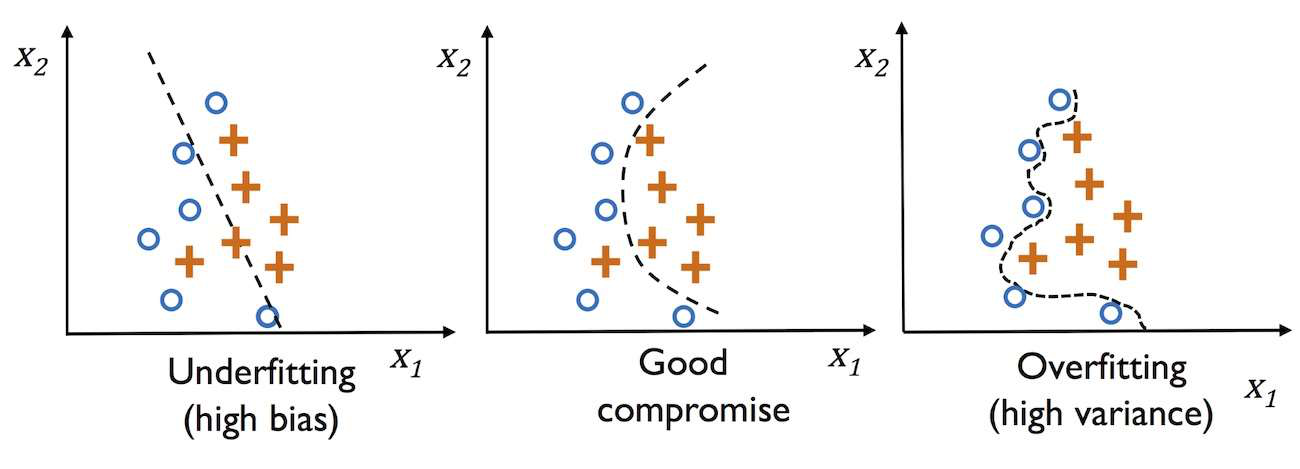
\includegraphics[width=11cm]{./images/p112_img523.png}
    \caption{Overfitting and underfitting}
\end{figure}

\noindent Bias refers to the error that is introduced by approximating a real-world problem with a simpler model, while variance refers to the error that is introduced by model sensitivity to small fluctuations in the training data.\\
Bias formula example:

A high-bias model may have poor performance on the training data but generalizes well to new data, while a high-variance model may have good performance on the training data but poor generalization performance.\\
\begin{figure}[!ht]
    \centering
    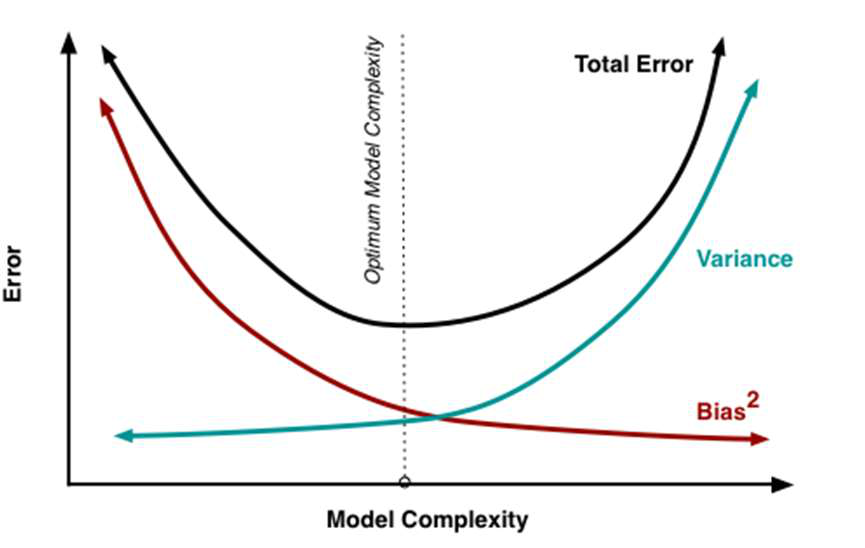
\includegraphics[width=11cm]{./images/p118_img552.png}
    \caption{Bias-variance tradeoff}
\end{figure}

\noindent One way to address the bias-variance tradeoff is through regularization techniques, which penalize the complexity of the model and encourage it to generalize better to new data. Another way is to use ensemble methods, such as bagging and boosting, which combine multiple models to reduce the variance and improve the generalization performance.


\end{document}